\documentclass[utf8, hyperref]{book}
\usepackage{titletoc}
\usepackage{titlesec}
\usepackage{ctexcap}
% \usepackage[b5paper,text={125mm,195mm},centering,left=1in,right=1in,top=1in,bottom=1in]{geometry}
% a4paper,top=0.9cm,left=2cm,bottom=0.9cm,right=2cm,includehead,includefoot
\usepackage[a4paper]{geometry}
\usepackage{imakeidx}
\usepackage{multicol}
\usepackage{hyperref}
\usepackage{url}
\usepackage{shorttoc} % 用来生成不那么繁琐的目录
\usepackage{amsfonts, amssymb}
\usepackage{graphicx}
\usepackage{amsmath}

\makeindex

\bibliographystyle{plain}

\begin{document}

\title{斯坦福CS224N汉语笔记 \\ Stanford CS224N Note in Chinese}
\author{Chong \\ Contact me at \url{zhangchong.july08@gmail.com}}
\date{\today}

\frontmatter

\maketitle
% \include{nonchap_前言.tex} % as a chapter
% \renewcommand\contentsname{目录}
\tableofcontents
% \shorttableofcontents{目录}{1}


\mainmatter

% 尽量不要用part,没必要空一页

% \part{总论}
\chapter{依存句法分析 \\ Dependency Parsing}

\small{讲师:Christopher Manning, Richard Socher}

\small{作者:Lisa Wang, Juhi Naik, and Shayne Longpre}

\small{讲义来源:\cite{04-this_notes} 额外参考:\cite{04-this_slides}}

% 句法分析(Parsing, Syntax Analysis)就是1.句子由词语组成,2.词语具有语法功能。

% \begin{multicols}{2}

\section{依存语法和依存结构 \\ Dependency Grammar and Dependency Structure}

\subsection*{成分语法和依存语法 \\ Constituency Grammar and Dependency Grammar}

用树状结构表示句子语法结构的想法是自然的,形成的树称为句法树(Parse Tree)。编译原理中的句法树展示形式语言的语法结构,而NLP中的句法树展示自然语言的语法结构。
常用的句法树结构有两种:成分语法(Constituency Grammar)和依存语法(Dependency Grammar)。

成分语法使用嵌套表示句子语法结构,和编译原理中基于产生式的文法很像。各级语法层次通过规约向上整合,形成句子的不同成分(Nested Constituent),并构成句子。本节不涉及这个概念,欲详细了解可以参考\ref{Constituency Grammar},并建议参考\cite{04-phrase-struct-gram}和\cite{04-this_slides}。

依存语法展示了词之间的二元不对称关系,即依存关系,用三元组表示为$(Head, r, Dependent)$,两个实体分别指代被依赖者和依赖者;用单向弧表示为$Head\stackrel{r}{\to}Dependent$.以下简单列举几种依存关系:

\begin{itemize}
    \item 修饰关系,某个词修饰另一个词。依赖者是修饰词(Modifier),被依赖者是被修饰词(Governor)。比如the beautiful girl,修饰词是beautiful,被修饰词(主语)是girl,所以beautiful依存于girl.
    \item 主次关系,一系列词具有相同地位,用第一个词占根节点位;或者某个成分有同位语,此时同位语依存于这个词。依赖者是下级(Inferior),被依赖者是上级(Superior)。
    \item 从属关系,某个词从属另一个词。依赖者是从属词(Subordinate),被依赖者是支配词(Regent)。
\end{itemize}

在具体分析句子的时候,一般先通过语法关系定义依存的不同种类,再确定每一处依存属于什么种类。
\cite{04-blog1}给出了更多、更精确的依存关系实例。从中可见,依存关系基本上是根据语法关系(主谓宾,同位语等)和句子成分(主语、介词宾语、同位语等)定义或设计的。然而,依存关系并不像成分语法那样一丝不苟地遵循自然语言语法设计关系:依存关系不强求和自然语言语法的严格对应,而是优先从方便计算机处理、方便标注数据等等因素来考虑,比如保证定义明确无歧义等等。因此,依存语法在确切语言学对应、关系直观性等human-friendly的方面可能稍逊于成分语法,但在表示难度、处理难度等属于process-friendly方面的因素表现更优。因此,目前大部分的句法分析数据集都是基于依存分析搭建的,而大多数较为成功的模型也是基于依存分析数据集提出的。

在依存的确切种类定义好之后,依存分析问题就是一个clearly-defined的计算机问题了。现在已经有了一些解决依存分析的工具,\cite{04-blog2}中介绍了一些应用实例。

\subsection{依存句法分析 \\ Dependency Parsing}

\subsubsection{依存树 \\ Dependency Tree}

依存树(Dependency Tree)就是以一个树状结构表示句子内部所有词的依存关系。在依存树中,依赖者作为被依赖者的子节点,通过依存关系连成树(有向图),如图\ref{04-tree}所示。

\begin{figure}[!htbp]
\centering
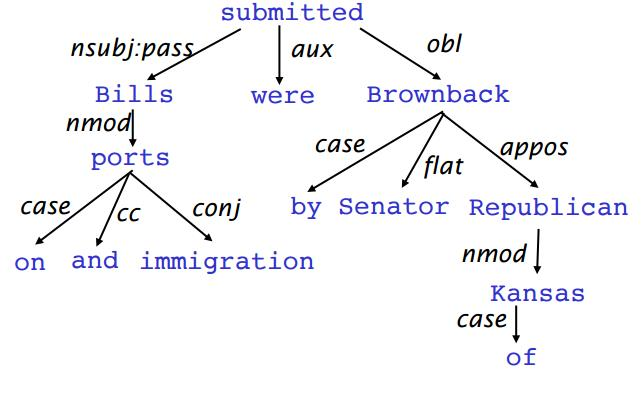
\includegraphics[width = 0.6\textwidth]{chap-04/04-01.jpg}
\caption{句子“Bills on ports and immigration were submitted by Senator Brownback, Republican of Kansas”的依存分析树。被依存者指向依存者,有向边上标识的属性是依存关系类型。}
\label{04-tree}
\end{figure}

有的时候会设置一个空节点充当这棵树的根节点,从而使句中的每一个词都依存于某个词。此时,可以用$S = (w_0w_1\cdots w_n)$表示一个句子,其中$w_0$是位于句首的空词语。
另外,在这种情况下,可以用两个和原句等长的序列表示依存树,一个序列确定被依赖词,一个序列确定是哪个关系。依存关系树可以用这种方式便利地表达出来。

\textbf{依存分析和句法分析的区别}

句法分析的核心是一步一步地解释句子展开成哪些成分,这些成分属于什么类型,然后再继续展开这些成分,自顶向下地把句子结构讨论清楚,并通过诸层次的展开关系来描述句子语法结果;而依存的分析方式并不是自顶向下的,也不需要把词汇本身的概念抽象出来,只是单纯展示句子中词语和词语之间的关系。
如前文所述,依存分析的结构更适合计算机处理\footnote{如上文所述,树状结构可以用两个序列表示,比嵌套结构表示起来方便一些,从而易于融入到通用的模型中。},同时也为人类保留了数据集的可读性(依存树也有一定的人类可读性),所以目前相对通常的句法分析/短语结构文法分析有优势。
关于短语结构文法/句法分析和依存语法分析的区别,建议阅读\cite{04-cnblogs2},讲的很详细。\cite{04-blog1}也点明了两者的区别。

关于自然语言的语法结构分析,还有很多新颖或实用的方法,比如普遍文法(或通用文法,Universal Grammar),旨在分析不同语言之间的共性成分,从而创建一个可以处理多种语言的大一统系统\footnote{相关资料可参考 \cite{04-uni1, 04-uni2, 04-uni3, 04-uni4}。}。

\subsubsection{依存句法分析的任务 \\ The Dependency Parsing Problem}

依存句法分析的任务是,输入句子$S$,输出依存句法树$G$. 这个任务分两部分(by Kuebler):

\begin{enumerate}
    \item 学习:给定数据集$D$(句子+句法树),训练模型$M$;
    \item 句法分析:使用这个模型进行预测,$G = M(S)$.
\end{enumerate}

在这方面,目前最流行的方法肯定是深度方法。

\subsection{基于状态转移的依存分析 \\ Transition-Based Dependency Parsing}

Transition-Based是一种做依存分析的思想,具有如下特点:

\begin{itemize}
    \item 数据集:每个句子的标签是从这个句子一步一步解析成依存分析树的状态转换序列。
    \item 模型效果:对于训练好的模型,输入句子当前的解析状态,输出下一个解析状态。所以预测模型是 一步一步地把整个句子的依存分析树解析出来。
\end{itemize}

因为依存分析的数据集在大多数情况下并不基于一个文法,所以不能给出一个明确的规约-展开规则,所以大部分Transition-Based的模型也并不需要依赖一个特定文法\footnote{也有基于成分分析搭建的模型,通过学习学到文法规则的使用策略(在给定的一组产生式中,在什么情况下优先用哪个产生式推导),然后通过这个策略逐步预测句子的推导过程。这种模型大多很麻烦,在此不多介绍。}。

\subsection{基于贪心方法的状态转移依存分析 \\ Greedy Deterministic Transition-Based Parsing}

根据上一节提出的Transition-Based思想,介绍(Nivre, 2003)模型,Nivre在2009年发表的综述\cite{04-NivreP}给出了这个模型的明确形式化定义。
对于用Transition-Based模型解决依存分析,这个模型实际上是将问题完全形式化,明确定义了Transition-Based模型应该具有的形式。

(Nivre, 2003)并不基于文法,而是基于一个有存储的状态机\footnote{形式语言的定义有两种主要途径,用文法定义或用状态机定义。\cite{04-tj}},定义如下:

\textbf{状态}

符合$c = (\sigma, \beta, A)$的三元组。其中:

\begin{itemize}
    \item $\sigma$表示一个栈,内部存储的元素是句子里的单词。
    \item $\beta$表示一个缓冲区,存储句子里的单词,对应尚未读入的单词。
    \item $A$表示句子中已经解析出来的依存关系的集合,其内部的元素形式为$(w_i, r, w_j)$,表示目前已经知道句子中$w_i, w_j$这两个词语之间具有$r$关系。
\end{itemize}

\textbf{初始状态和终止状态}

\begin{itemize}
    \item 初始状态:状态机只读入了句首的空单词,其他单词都还没读入,也没有任何依存关系被解析出来。
    $c_0 = ([w_0]_\sigma, [w_1, \cdots, w_n]_\beta, \emptyset)$.
    \item 终止状态:所有单词都读入,且栈中只剩根节点(特地加入的空节点,位于句首)的状态。
    $F = \{c_f\}, c_f = ([w_0]_\sigma, []_\beta, A)$.
\end{itemize}

\textbf{转移}

(Nivre, 2003)定义了三种状态转移:

\begin{itemize}
    \item $Shift$:在缓冲区非空的情况下,将缓冲区的第一个单词入栈。
    $(\sigma, w_i|\beta, A)\to(\sigma|w_i, \beta, A)$.
    \item $Left-Arc_r$:解析出依存关系$(w_j, r, w_i)$,其中$w_j$是栈顶,$w_i$是栈顶的第二个元素。在添加这个依存之后,$w_i$出栈。要求栈内至少有两个元素,且$w_i$不能为根节点。
    $(\sigma|w_i|w_j, \beta, A)\to(\sigma|w_j, \beta, A|\{r(w_j, w_i)\})$.
    \item $Right-Arc_r$:解析出依存关系$(w_i, r, w_j)$,其中$w_j$是栈顶,$w_i$是栈顶的第二个元素。在添加这个依存之后,$w_j$出栈。要求栈内至少有两个元素,且$w_i$不能为根节点。
    $(\sigma|w_i|w_j, \beta, A)\to(\sigma|w_i, \beta, A|\{r(w_i, w_j)\})$.
\end{itemize}

不难发现,对于任意一种状态,对其进行上述三种变换中的一种,所能得到的状态是唯一的:三种变换都是单值函数。也就是说,在给定当前状态时,Transition-Based模型用于在三种变换中正确决策。本节标题中提到的“贪心”正是点明这一点,模型不断对下一步转移进行判断,然后转移到下一个状态,至终止状态为止。

Nivre的工作还有很多,他自己在2019年也进行了总结,可以参考\cite{04-NivrePaper, 04-NivreSlides}.

\subsection{神经依存分析 \\ Neural Dependency Parsing}

本节在上一节基于贪心策略的Transition-Based模型基础上,介绍神经网络/机器学习/深度学习在其中的应用。如上一节所述,基于贪心策略的模型只需要在给定当前状态时做出下一步转移的决策(这实质上是一个分类问题),依决策移动到下一个状态,并最终解析出整个句子的依存关系。
在深度学习时代,我们在预测下一步转移时使用神经网络做分类,模型分为如下两步:

\textbf{特征选择}

基于特征选择的依存分析模型称为Feature-Based Discriminative Dependency Parsers,这类模型不直接用状态的完整信息做分类,而是通过一些预先定义的规则提取部分特征,并只参考这些特征的信息进行分类。在分类环节也不一定只使用神经网络模型,可能会基于一些简单统计或其他模型。

特征选择的环节就是在给定当前状态下,模型按规则从状态中提取若干特征,再根据特征形成模型的输入向量。一般提取的特征包括:

\begin{itemize}
    \item $S_{word}$:句子中的部分单词,用词向量的形式表示。这些单词一般是栈顶的几个单词或缓冲区即将被读入的前几个单词。使用单词的个数记为$n_w$.
    \item $S_{tag}$:一部分单词对应的词性(Part of Speech, POS)标签。使用词性标签的个数记为$n_t$.
    \item $S_{label}$:句子中存在的部分依存关系。前文提到,可以用两个和原句等长的序列表示句法树,一个序列确定被依赖词,一个序列确定是哪个关系;所以在此处,对于特定词语的依存关系,也用“被依存词+依存关系类型”来表示。关系的个数记为$n_l$.
\end{itemize}

\begin{figure}[!htbp]
\centering
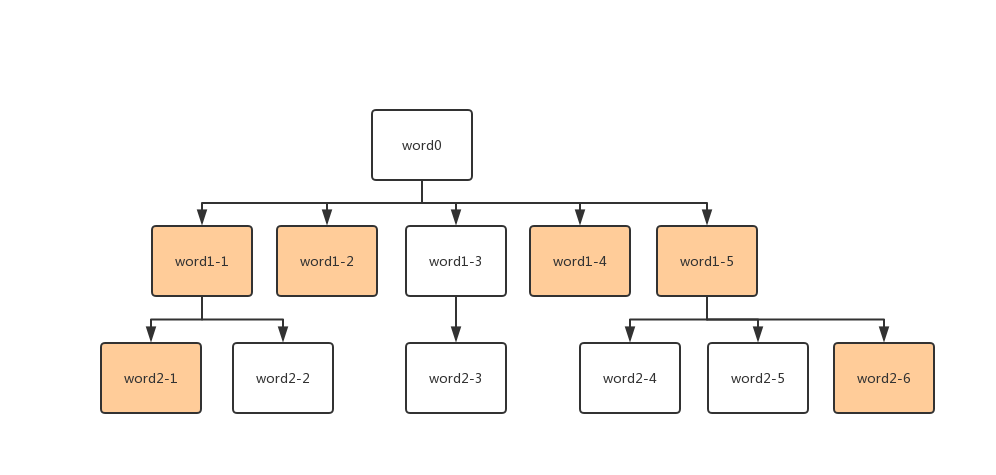
\includegraphics[width = 0.7\textwidth]{chap-04/consider-which-six.png}
\caption{在依存分析中,和栈顶词相关的需要考虑的词。图中$word_0$(根节点)表示栈顶前两个词中的一个,标黄的词表示与这个词相关的需要考虑的词,一共有6个。}
\label{04-consider-which-six}
\end{figure}

例如:

\begin{itemize}
    \item $S_{word}$:使用栈顶的前3个词,缓冲区即将被读出的前3个词;对于栈顶的前2个词,使用其最左/最右各2个子节点,及其最左/最右子节点的最左/最右子节点,如图\ref{04-consider-which-six}所示。$n_w = 3 + 3 + 2 * 6 = 18$.
    \item $S_{tag}$:上述单词对应的词性标签,$n_t = 18$.
    \item $S_{label}$:除了栈顶的前3个词和缓冲区即将被读出的前3个词之外,其余12个词的依存关系,即以这些词为依赖者的依存关系。$n_l = 12$.
\end{itemize}


\textbf{模型}

经过特征选择之后,模型的输入由三部分组成:词用本词的One-Hot向量表示,词性标签用本标签的One-Hot向量表示,依存关系用本关系的One-Hot向量和被依存者这个词的One-Hot向量表示。这些One-Hot向量的维数分别为词典长度,词性标签的种类数和依存关系的种类数,所以输入向量很稀疏。
稠密表示一直是深度模型的传统优点。在上述特征输入模型时,模型中的嵌入层将每个One-Hot向量编码成一个$d$维的向量,实现了特征向量的稠密表示。
具体而言,和大多数工作一样,这里介绍的简单模型中的嵌入层就是一个线性变换。因为输入的是One-Hot向量,所以其实这个线性变换的实质就是取内部系数矩阵的某一列。这个系数矩阵称为嵌入矩阵,实际上包含了所有词/标签/关系的嵌入向量。目前常用的词嵌入工具就是训练一个带嵌入层的模型,然后把里面的嵌入矩阵拿出来当词向量使用。

\begin{figure}[!htbp]
\centering
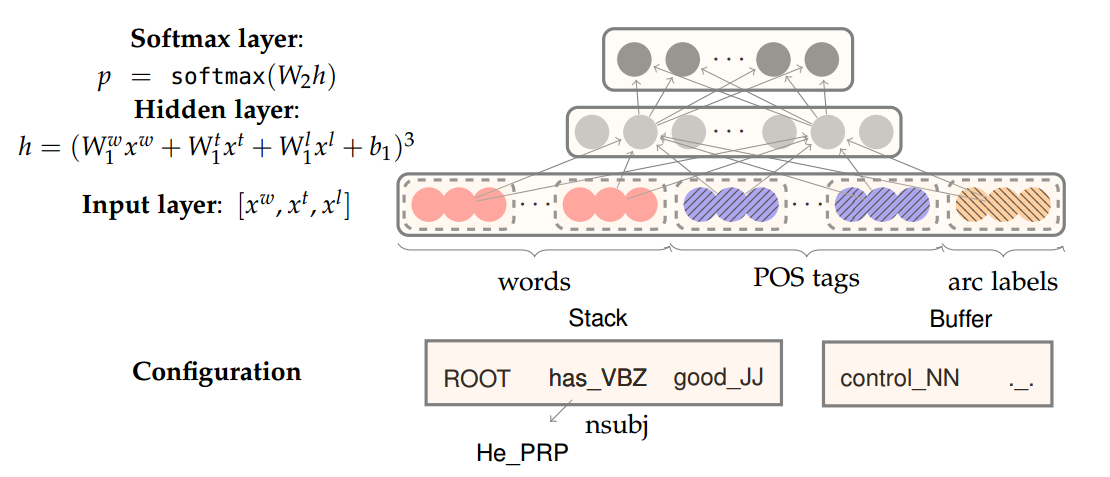
\includegraphics[width = 0.8\textwidth]{chap-04/04-model.png}
\caption{一个简单的神经网络,用来决策转移动作。网络依次包括嵌入层/输入层、隐层和softmax输出层。}
\label{04-net}
\end{figure}

模型最基础的结构如图\ref{04-net}所示。输出向量的维度和转移操作的种类数对应(3维),指出应该采取哪种转移。\cite{04-manning}提出了更复杂的网络结构。在Transition-Based依存分析方面也有很多丰富的思考,比如\cite{04-cnblogs1}等等。
随着深度学习的发展,使用深度学习解决依存分析问题的探索层出不穷,笔者在此列举的资料也只是管中窥豹,仅做参考。

% \end{multicols}

\section{章节附录}

\subsection{成分语法 \\ Constituency Grammar}
\label{Constituency Grammar}

成分语法的思路就是设计一套文法,和实际的自然语言语法形成密切对应。在相关的研究中,成分语法、短语结构文法(Phrase Structure Grammar)和上下文无关文法(Context Free Grammar)通常指代相同的概念,即用产生式文法的观点来解析自然语言的语法结构。

具体而言,考虑自然语言中的各个层次,如词语、短语、成分、句子等,他们对应的抽象概念是词性、短语类型、成分类型和句子类型,这些不同层级、不同类型的概念之间的联系可以用产生式文法来体现。细节如下:

\begin{itemize}
    \item 词语:词语是句子语法解析的终点,同种词性的词语在句子中发挥的作用是相似的,而词性在产生式中充当终结符(或准终结符)。例如,在产生式$Adj. \ Modified \ N. \ Phrase \to Adj.+N.$中,可以设计成$N.$就是终结符,也可以设计成$N.\to apple | banana | \cdots$,而定义$apple$等词语为终结符。
    \item 短语:短语由更低级的单元(词语)组成,而本身也有特定意义(短语的语法结构),对应文法中的非终结符。例如,$Adj. \ Modified \ N. \ Phrase$的一个实例是$big apple$,$big$属于$Adj.$,$apple$属于$N.$
    \item 成分:和短语一样,成分也是“句子-成分-短语-词语”的语法层次中间的链结,对应非终结符。例如,名词短语$big apple$可以充当句子的主语$S.$.
    \item 句子:对应文法中的起始符号。
    \item 层次间关系:层次间关系可以用产生式描述。
    \begin{itemize}
        \item 词语组成短语:某一特定类型的短语可以由特定词性的词语按特定顺序组成,这种信息用产生式描述,比如$Adj. \ Modified \ N. \ Phrase \to Adj.+N.$
        \item 短语充当成分:产生式阐明句子成分由怎样的短语充当。比如$S. \to Adj. \ Modified \ N. \ Phrase$.
        \item 成分组成句子:产生式阐明句子的构成方法。比如$Sentence \to S. + Predicate + O.$.
    \end{itemize}
\end{itemize}

使用产生式文法描述这些概念的关系是很自然的思路,很好理解。将句子按文法规则进行规约,获得的语法树能清晰地体现句法结构。但是,成分语法难以应用于大规模数据集上句子语法结构的表示,原因如下:
\begin{itemize}
\item 语法树的嵌套结构没有直观的表示方法:依存关系树中的节点都是单词,所以可以用每个单词的被依存者表示整棵树;但成分语法树中单词都是叶子节点,按照层次聚合起来,所以不好表示。
\item 智能方法无法学习新的规则,所有的文法规则需要由人提前定义好。考虑到大规模语料的复杂性,靠人力编排规则难免有遗漏和不周之处,而且和NLP目前通用化、智能化的趋势背道而驰。
\end{itemize}
综上所述,在大数据时代,语法结构表示上的弱点限制了成分语法的进一步应用和发展,目前的应用范围远不及依存语法。目前句子结构分析的大部分数据集都是基于依存关系建立的。

不过,成分语法作为一个形式优雅、定义清晰的概念,还是有很大用处的。比如,在缺数据的时候可以用成分语法生成一些句子数据,然后用生成的数据集验证模型。根据具体的生成方式,这些句子实际上属于几个特定的类别,所以有一定复杂性,适合作为验证数据。

\section*{章节未尽之处}

\begin{thebibliography}{本章节参考文献\&阅读材料}
\bibitem[notes04]{04-this_notes} \url{https://web.stanford.edu/class/cs224n/readings/cs224n-2019-notes04-dependencyparsing.pdf}
\bibitem[lecture05]{04-this_slides} \url{https://web.stanford.edu/class/cs224n/slides/cs224n-2019-lecture05-dep-parsing.pdf}
\bibitem[Phrase Structure Grammar]{04-phrase-struct-gram} \url{https://www.thoughtco.com/phrase-structure-grammar-1691509}
\bibitem[依存分析:中文依存句法分析简介]{04-blog1} \url{https://blog.csdn.net/sinat_33741547/article/details/79258045}
\bibitem[依存句法分析:原理、应用]{04-blog2} \url{https://blog.csdn.net/qq_17832003/article/details/84396257}
\bibitem[Dependency Parsing的两种解决方案]{04-cnblogs1} \url{https://www.cnblogs.com/zeze/p/9752734.html}
\bibitem[Nivre's Paper]{04-NivrePaper} Nivre, Joakim. (2019). Inductive Dependency Parsing of Natural Language Text. 
\bibitem[Nivre's Slides]{04-NivreSlides} \url{https://www.docin.com/p-1736992284.html}
\bibitem[Danqi Chen and Manning's Paper of Neural Dependency Parsing]{04-manning} Danqi Chen, and Christopher D. Manning. "A Fast and Accurate Dependency Parser using Neural Networks." EMNLP. 2014.
\bibitem[Nivre's Summary]{04-NivreP} Kuebler, Sandra, Ryan McDonald, and Joakim Nivre. “Dependency parsing.” Synthesis Lectures on Human Language Technologies 1.1 (2009): 1-127.
\bibitem[依存句法分析与语义依存分析的区别]{04-cnblogs2} \url{https://www.cnblogs.com/CheeseZH/p/5768389.html}
\bibitem[统计自然语言处理]{04-tj} 统计自然语言处理(第2版),宗成庆,ISBN: 9787302165989,引用3.2.1的内容.
\bibitem[Universal Grammar in Wikipedia]{04-uni1} \url{https://en.wikipedia.org/wiki/Universal_grammar}
\bibitem[What is Universal Grammar?]{04-uni2} \url{https://www.sohu.com/a/223760135_652705}
\bibitem[Definition and Examples of Universal Grammar (UG)]{04-uni3} \url{https://www.thoughtco.com/universal-grammar-1692571}
\bibitem[普遍语法假说学习汇报]{04-uni4} \url{https://wenku.baidu.com/view/654273093a3567ec102de2bd960590c69ec3d80f.html}
\end{thebibliography}



\chapter{语言模型和RNN \\ Language Models}

\small{讲师:Christopher Manning, Richard Socher}

\small{作者:Milad Mohammadi, Rohit Mundra, Richard Socher, Lisa Wang, Amita Kamath}

\small{讲义来源:\cite{05-this_notes} 额外参考:\cite{05-this_slides, 05-this_slides2}}

本章默认读者已经掌握RNN, GRU, LSTM的理论知识,涉及RNN的部分只谈应用。关于RNN, GRU, LSTM的理论知识在后期会在附录补充。

% \begin{multicols}{2}

\section{语言模型 \\ Language Models}

\subsection{介绍 \\ Introduction}

\textit{笔者强烈建议阅读\cite{05-tj-qk},这本书对语言模型的介绍恰到好处,比CS224N讲义或我的笔记写得都好。CS224N内容太少且过于跳跃,而我的笔记为了对应原来讲义的标题和内容,逻辑性更差。}

语言模型(Language Model)是NLP中\textbf{预测下一个词语}的任务,给出当前句子的所有前文,模型需要预测下一个出现的词语是什么。

从数学上说,就是给出$P(x_{n+1}|x_1 = w_{i_1},\cdots,x_n = w_{i_n})$,即前$n$个词确定时$x_{n+1}$的分布律。其中,$x_i$表示句子中第$i$个词,$w_i$表示词库中的第$i$个词。

从另一个角度看,语言模型给出词序列出现的概率。记$P(w_1, \cdots, w_m) = P(x_1 = w_1, \cdots, x_m = w_m)$为词序列$\{w_1, \cdots, w_m\}$作为一个句子出现的概率\footnote{“作为一个句子出现”指的是,这个句子正好就是这个词序列。比如我们有一个未知的句子由5个单词构成,上述公式可以给出这个句子恰好是"I have a big dog."的概率。},则有
\begin{equation*}
\label{gram-raw}
P(w_1, \cdots, w_m) = \prod_{i=1}^{i=m}{P(w_i | w_1, \cdots, w_{i-1})}
\end{equation*}
对这个公式的理解:一方面,这个公式就是按条件概率展开得到的;另一方面,每一项的条件概率表明预测当前词时,参考概率由上文给定,每个词的判断都是参考全部上文进行的。

\subsubsection{N元语法 \\ N-Gram Language Models}

基于n元语法的语言模型对上述公式进行了改良。在预测第$i$个词$w_i$的出现概率时,只考虑这个词之前的$n$个词,即$w_{i-n}, \cdots, w_{i-1}$.形象地,我们认为有一个$size = n$的窗口(Window)在计算概率/预测当前词的过程中跟随当前位置移动。我们在计算概率/预测当前词时只考虑窗口内的词作为上文。

\begin{equation}
\label{n-window}
P(w_1, \cdots, w_m) \approx \prod_{i=1}^{i=m}{P(w_i | w_{i-n}, \cdots, w_{i-1})}
\end{equation}

这样做的好处是不言而喻的:原公式中,每个词的预测都需要参考全部上文,上文是变长的;在公式\ref{n-window}中,我们用窗口限制上文的长度,上文是定长的,从而情况数是固定的,而且更容易列举。此外,基于n元语法的模型减少了上文的情况数,从而改善了稀疏性问题和存储问题。关于这两个问题,在章节\ref{n-gram}详细讨论。

公式\ref{n-window}在Seq2Seq任务比较常用。以机器翻译为例,在对短语/句子给出翻译结果之后,系统一般会基于规则给出一系列相近的翻译结果。基于公式\ref{n-window},可以建立评价指标,从而判断这些结果中哪个最好。
\begin{itemize}
    \item 例如,对于汉语“我有一只猫”给出翻译"I have a cat",通过规则(比如选取同义词,调整词序)生成数个备选翻译"I has a cats", "Me have the cat", "Me had cats", "I have a dog", "Have I a cat"等等。
    \item 建立评价指标,判断这些翻译的得分,输出得分最高的翻译。我们对于评价指标具有如下期望:
    \begin{itemize}
        \item 因为"I have a cat"是正确的翻译,所以我们希望"I have a cat"的得分比其他备选项高,从而使得"I have a cat"作为正确的翻译被输出。
        \item 因为乱序比主格宾格/人称形式错误更影响阅读,所以我们希望"Have I a cat"的得分比"Me have the cat"或者"I has a cats"更低。
        \item 因为词意错误比其他错误更影响阅读,所以我们希望"I have a dog"的得分比"Me have the cat"这种句子更低。如果是"You have a dog",评分更低。
        \item …
    \end{itemize}
    诸如此类,这些期望都是很主观的。评分标准是程式化的,在很多情况下完全依赖于公式\ref{n-window}所计算的概率,但好的评分标准能够在易于实现的基础上照顾到人的需要。
\end{itemize}

\subsection{基于N元语法计算条件共现频率 \\ Calculation Prediction Probability in N-Gram Based Language Models}
\label{n-gram}

\subsubsection{基于N元语法计算条件共现频率}

上一节提到了基于n元语法的语言模型,用窗口限制上文长度。实际上n元语法还有另一个核心思想:用n元词组,即n个连续单词的块解析句子。
例如,用4-gram将句子"Mary had a little lamp whose fur is white as snow."分为"Mary had a little", "had a little lamp", "a little lamp whose", ..., "is white as snow".
在这种思想基础上,通过统计不同的词组出现频率,计算条件概率。首先,统计$\leq$n元词组所有可能情况的共现(Co-Occurance)次数;然后,对于特定的词语出现概率,通过对应的共现次数相除计算,得到在前$n-1$个单词固定情况下第$n$个单词的可能情况。

\begin{equation*}
\begin{aligned}
P(w_i | w_1, \cdots, w_{i-1}) & = & P(w_i | w_{i-n}, \cdots, w_{i-1}) & \ \ \mbox{限制上文长度}\\
 & = & \frac{P(w_{i-n}, \cdots, w_{i})}{P(w_{i-n}, \cdots, w_{i-1})} & \ \ \mbox{条件概率展开}\\
 & = & \frac{count(w_{i-n}, \cdots, w_{i})}{count(w_{i-n}, \cdots, w_{i-1})} & \ \ \mbox{频率代替概率}
\end{aligned}
\end{equation*}

如上面公式所示,核心思想是用n元词组的共现次数(频率)代替n元词组的出现概率。

公式\ref{bi-gram}和\ref{tri-gram}是计算条件概率$P(w_i | w_{i-n}, \cdots, w_{i-1})$的两个实例,分别对应二元语法(Bi-Gram)、三元语法(Tri-Gram)的情况。

\begin{equation}
\label{bi-gram}
p(w_{i + 2} | w_{i + 1}) = \frac{P(w_{i + 1}, w_{i + 2})}{P(w_{i + 1})} = \frac{count(w_{i + 1}, w_{i + 2})}{count(w_{i + 1})}
\end{equation}

\begin{equation}
\label{tri-gram}
p(w_{i + 3} | w_{i + 1}, w_{i + 2}) = \frac{P(w_{i + 1}, w_{i + 2}, w_{i + 3})}{P(w_{i + 1}, w_{i + 2})} = \frac{count(w_{i + 1}, w_{i + 2}, w_{i + 3})}{count(w_{i + 1}, w_{i + 2})}
\end{equation}

\subsubsection{预设参数n对n元语法模型的影响}

N元语法的本质是参考前n个单词选择当前单词,所以n的值会影响选择效果。
如果n的值太小,参考的上文信息不足,导致判断正确率下降;有时甚至无法追溯到决定词汇选择的信息,从而没有机会做出正确选择。从信息量的观点考虑,肯定希望n的值尽量大。
然而,如果n的值太大,如下两点问题将会成为模型的瓶颈:

\textbf{稀疏性问题}

稀疏性问题指的是在形如公式\ref{bi-gram}, \ref{tri-gram}中,分子或分母为0的情况。在n值增大时,大多数词语组合在数据集中没有出现过,所以会经常出现这种情况。
此问题有如下解决方法:

\begin{itemize}
    \item 平滑处理(Smoothing):加一个平滑项$\delta$于分子、分母上,主要防止分子为0.$P = \frac{count(**)}{count(*)}\to\frac{count(**)+\delta}{count(*)+\delta}$.
    \item 退避(Backoff):如果窗口大小为n时分母为0,那么就把窗口大小减为n-1,以此类推,至已经有相应的前缀,分母不为0即可。退避的主要作用是防止分母为0.$P = \frac{count(w_{i + 1}, w_{i + 2}, w_{i + 3})}{count(w_{i + 1}, w_{i + 2})}\to\frac{count(w_{i + 2}, w_{i + 3})}{count(w_{i + 2})}$.
\end{itemize}

稀疏性问题从表面上看是因为样本量太小造成的,但实际上是因为n元词组的情况数太多而造成的,增大样本量并不能显著改善稀疏性问题。上述的两种处理方式,前者是一个数值分析领域经常采取的平滑思想,后者是试图动态调整n的手段。

\textbf{存储问题}

状态数和元数n是指数关系,较大的元数会使状态数产生爆炸现象,从而无法提供那么多空间存储统计数据。

存储问题的本质实际上和稀疏性问题一样:在相同的问题下,数据规模恒定,所以各种情况的总和是确定的;情况数增加,则有更多的情况样本数少/没有样本,造成统计学上的不可靠/不稳定。总之,稀疏性问题和存储问题出现的根本原因都是情况数太多,而n元语法减少了情况数,缓解了这一问题。在\cite{05-tj-qk}中说了这件事。

合适的n值既能照顾到上述两点问题,又不至于依据太少的信息进行计算。一般$n<5$.

从上述的两点问题也能看出n元窗口机制的优越性:有效地限制了情况数(状态数),缓解了上述两大问题。如果使用变长条件计算条件概率,记句子的最长长度为$m$(一般$m>>n$),那么$\leq m$元的所有可能词组都要列入情况。而状态数和元数是指数关系,较大的元数会使状态数产生爆炸现象。另外,大部分词组完全不可能作为句子开头,存之无用,造成冗余。

\subsubsection{N元语法模型的评价}

N-gram以及类似的统计模型确实在工程上取得了巨大的成功,比如(已经在10年前被各种文献资料引用无数遍的)朴素贝叶斯模型在垃圾邮件判别上的应用。
但是,\cite{05-stat-fail}等资料已经指出了统计模型的诸多缺点:
\begin{itemize}
    \item 统计模型完全不符合人类的判断逻辑。N-gram模型的判断是基于前文的n个单词,但人类完全不会这么做:人类的思维过程是先决定表达什么语义,然后映射到一个语法树结构,然后再选词。
    \item 作为非智能方法,统计模型在数据量日益增加的趋势下,效果不及智能方法,尤其是深度方法。
\end{itemize}

\subsection{基于窗口的语言模型 \\ Window-based Neural Language Model}

上文所述的稀疏性问题和存储问题都属于机器学习中“维度灾难”(Curse of Dimensionality)问题,关于此概念,更多内容见\ref{curse}. 维度灾难问题在基于统计的模型中屡见不鲜。
然而,随着深度学习大行其道,很多原有模型面临的维数灾难的问题已经解决。

\begin{itemize}
\item 用One-Hot向量表示词语就是一个容易受到维数灾难影响的方法,随着语料规模的增加,词语的总个数增加,向量维度增大(而且内容稀疏),导致模型的效果弱化;而用深度学习训练的词嵌入模型为词语提供了低维度的嵌入表示,从而改善了这个问题。
\end{itemize}

在这方面,最早的工作是Bengio在2003年发表在NIPS上的\cite{05-bengio03},最经典的工作是Word2Vec\footnote{Word2Vec已经工具化,参考\cite{05-w2v}.}\cite{05-w2v-model, 05-w2v-opti}.
上述工作作为神经语言模型早期的工作,孕育了window context思想和window-based模型,即每个单词的前后各n个单词作为这个单词对应的上下文,在判断这个单词时使用,其中n为窗口大小。
Window-based模型从提出到现在,被NLP整个领域广泛采纳,已经取得了极大的成功。

\section{循环神经网络(RNN)的应用 \\ Application of RNN}

\textit{在阅读本节之前,默认读者已经掌握RNN的理论知识,如模型构造和思想等。}

\begin{figure}[!htbp]
\centering
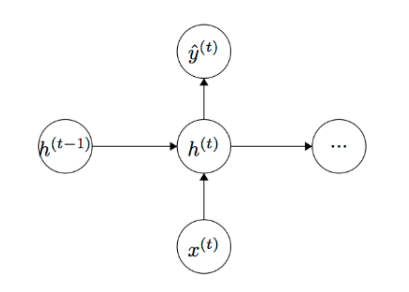
\includegraphics[width = 0.4\textwidth]{chap-05/05-RNN.png}
\caption{RNN单元的输入输出结构}
\label{05-RNN}
\end{figure}

上一节所述的window-based模型在很长一段时间内是主流的语言模型。然而,随着2015年RNN-based模型的兴起,后者已经逐渐取代前者成为主流。当然,长江后浪推前浪,在2019年学术界的兴趣已经转向Attention/Transformer-based模型了。

RNN-based模型的最大特点是对上下文信息的扩充。Window-based模型只能考虑有限大小的上下文,然而RNN-based模型具有记忆性,使用的上下文信息是该句在这个词之前的所有部分\footnote{如果是双向RNN,则上下文是这个单词的所有前后文,包括本句的所有信息。},相比window-based模型具有更大的信息量,所以理论上更能够判断正确。

\begin{figure}[!htbp]
\centering
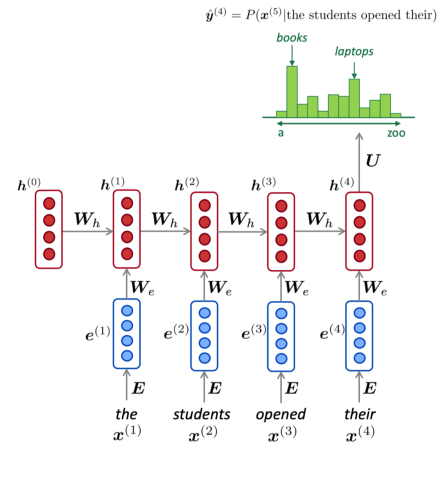
\includegraphics[width = 0.5\textwidth]{chap-05/05-prediction.png}
\caption{RNN可以用于文本生成。}
\label{05-prediction}
\end{figure}

RNN模型经常使用交叉熵和困惑度作为评价指标。对上述概念,\cite{05-tj}讲的很详细。

\subsection{RNN语言模型的特点 \\ Advantages, Disadvantages and Applications of RNNs}

\textbf{优点}

\begin{itemize}
    \item 可以处理变长输入,且模型体量不随输入序列长度增加而增加。RNN对变长的适应性是天然的,不需要做额外的调整,因而在相关问题(比如NLP问题)中一直很受重视。
    \item 具有记忆,可以认为当前词语是基于全部前文决定的。这一点也是RNN相对window-based模型的显著优点。
    \item 所有的输出都通过一组相同的参数计算而得,可以认为预测过程具有普遍性。
\end{itemize}

\textbf{缺点}

\begin{itemize}
    \item 并行程度低,不方便计算。这个问题没法解决,Attention在2017年问世之后逐渐取代RNN也和并行计算方面的因素有关。
    \item 短期记忆问题:因为梯度消失等问题,RNN的记忆性不够,过于靠前的前文对当前词语的判断已经影响不大。\ref{05-solution-vanish}介绍了一些对策。
\end{itemize}

\textbf{内存占用}

运行一层RNN所需的内存量与语料库中的单词数以及句子中的单词数成正比,前者决定了输入One-Hot向量的维数,后者决定了内存中保存向量的个数。另外,内存中还需要保存两对$W, b$系数矩阵。

\subsection{梯度爆炸和梯度消失的对策 \\ Solution to the Exploding and Vanishing Gradients}
\label{05-solution-vanish}

\textbf{梯度爆炸}

梯度爆炸的典型对策是梯度修剪,即当梯度值大于上限阈值时,用一个上限值代替之。

这个方法很朴素,但很有效。如图\ref{05-wall}所示,当在一个如图所示的误差面上训练时,误差本来在平稳地下降(实线箭头),但突然遇到一个梯度极高的地方(高误差壁,High Error Wall),导致这一步梯度极大,导致当前位置的移动到一个极远的位置(实线大箭头),影响下降进度。利用梯度修剪可以让当前位置的移动没有那么远(虚线大箭头),在图中可以继续平稳下降(虚线小箭头)。


\begin{figure}[!htbp]
\centering
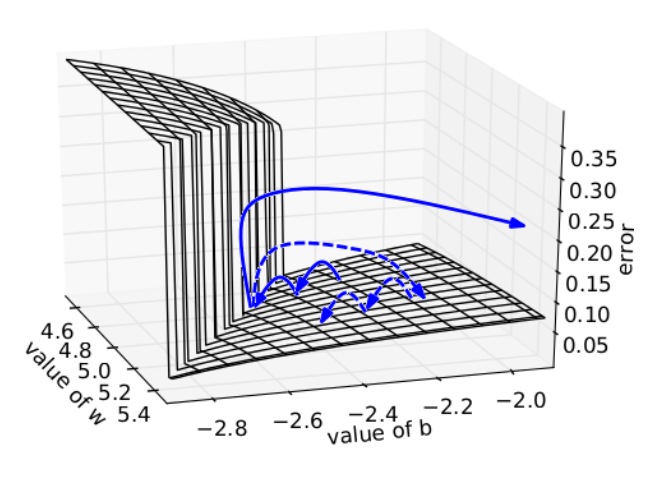
\includegraphics[width = 0.8\textwidth]{chap-05/05-wall.png}
\caption{梯度修剪缓解梯度爆炸问题的一个实证。}
\label{05-wall}
\end{figure}

\textbf{梯度消失}

梯度消失比梯度爆炸更需要控制,因为梯度爆炸会导致数据超过数据范围而报错,而梯度消失会使梯度数值降为0,在这种状况下,我们无法确定当前位置对前文是完全没有依赖,还是有依赖但因为距离太远,梯度已经消失。

梯度消失具有如下对策:

\begin{itemize}
    \item 系数矩阵的初始化不再随机,而是谨慎选取一个恰当位置;
    \item 使用ReLU作为激活函数:因为ReLU的导数不是0就是1,不存在导数$<<1$的状态,因而不会在反向传播的导数值相乘过程中出现梯度消失。
\end{itemize}

随着RNN各种变体的提出,无论是针对单元改进(LSTM),针对结构改进(双向、多层RNN网络)还是在思想上的改进(Encoder-Decoder),都在一定程度上解决了RNN网络短期记忆的问题,梯度爆炸和梯度消失对模型的影响已经逐渐成为历史。

\subsection{基于RNN的机器翻译 \\ Application: RNN Translation Model}

机器翻译领域的传统方法是统计机器翻译,但在深度学习出现之后,神经机器翻译已经体现出巨大的优势。
统计机器翻译(Statistical Machine Translation, SMT)的模型都把翻译分为很多阶段,每个阶段使用不同的方法和模型,整体非常复杂;而神经机器翻译(Neural Machine Translation, NMT)实现了机器翻译的端到端模型,模型简洁,效果突出。
NMT目前的workline主要有三个分支:基于CNN,基于RNN和基于Attention,目前似乎最后一者最火。我们在此主要介绍一些经典的和RNN相关的工作。

最简单的基于RNN的机器翻译模型通过一张图就能说清。如图\ref{05-rnn-nmt}所示。先前的时间阶段输入源语言句子,在源语言句子输入结束后,模型陆续生成目标语言的翻译。
图中在翻译过程中的输入是先前输出的翻译结果,这样能给翻译提供更多的信息。实际上输入其他向量也是可以的,有理由即可,效果另说。

\begin{figure}[!htbp]
\centering
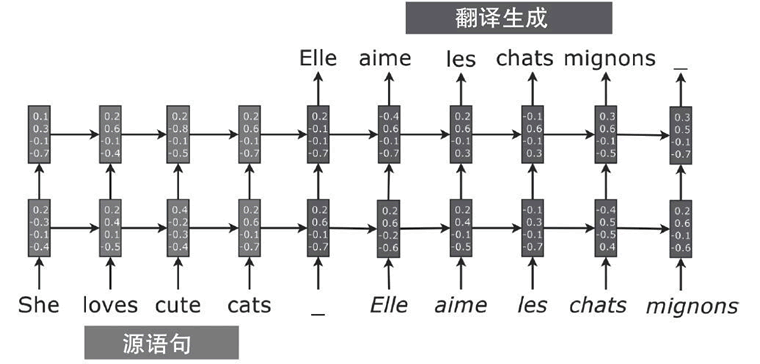
\includegraphics[width=0.8\textwidth]{chap-05/05-rnn-nmt.png}
\caption{最简单的基于RNN的机器翻译模型}
\label{05-rnn-nmt}
\end{figure}

对于这个简陋的模型,实际应用中又有如下改进:

\begin{itemize}
    \item 解码阶段和译码阶段的RNN单元使用不同的权重矩阵;
    \item 把上一个时段的预测输出$\hat{y}$也加入RNN单元的输入;
    \item 使用双向/多层RNN;
    \item 翻转输入序列(但不翻转输出序列)。
\end{itemize}

这些想法都很自然,提出的时候也有背书,而且也都取得了良好的结果。
% \end{multicols}

\section{章节附录}

\subsection{维数灾难 \\ Curse of Dimensionality}
\label{curse}

维数灾难指模型随着数据维数增大而出现问题,无法正常发挥作用的情况。

维数灾难的原理

维数灾难的实例

% 维度灾难
% 我们主要谈自然语言中的维数灾难,从理论和分类上谈,多举例子
% 理论 https://www.cnblogs.com/dingz/p/9029395.html
% 机器学习中的位数灾难 https://blog.csdn.net/qq_39521554/article/details/80653712
% 提到的Bengio论文 https://blog.csdn.net/hx14301009/article/details/80345449

\section*{章节未尽之处}

维数灾难待补

梯度爆炸和梯度消失的理论详解待充实,应该提炼出来放附录

RNN一套待补,其中原来讲义的图特别好,建议借鉴

\begin{thebibliography}{本章节参考文献\&阅读材料}
\bibitem[notes05]{05-this_notes} \url{https://web.stanford.edu/class/cs224n/readings/cs224n-2019-notes05-LM_RNN.pdf}
\bibitem[lecture06]{05-this_slides} \url{https://web.stanford.edu/class/cs224n/slides/cs224n-2019-lecture06-rnnlm.pdf}
\bibitem[lecture07]{05-this_slides2} \url{https://web.stanford.edu/class/cs224n/slides/cs224n-2019-lecture07-fancy-rnn.pdf}
\bibitem[On Chomsky and the Two Cultures of Statistical Learning]{05-stat-fail} \url{http://norvig.com/chomsky.html}
\bibitem[A Neural Probabilistic Language Model]{05-bengio03} \url{http://www.jmlr.org/papers/volume3/bengio03a/bengio03a.pdf}
\bibitem[Word2Vec in gensim]{05-w2v} \url{https://radimrehurek.com/gensim/models/word2vec.html}
\bibitem[Word2Vec CBOW and Skip-Gram]{05-w2v-model} Efficient Estimation of Word Representations in Vector Space, Tomas Mikolov et al, \url{https://arxiv.org/abs/1301.3781}
\bibitem[Word2Vec Optimization]{05-w2v-opti} Distributed Representations of Words and Phrases and their Compositionality, Tomas Mikolov et al, \url{https://arxiv.org/abs/1310.4546}
\bibitem[统计自然语言处理]{05-tj} 统计自然语言处理(第2版),宗成庆,ISBN: 9787302165989,引用2.2.5, 2.2.6, 5.2的内容,这三节分别介绍了交叉熵的定义、困惑度的定义和两者在语言模型中的应用,言简意赅。
\bibitem[统计自然语言处理]{05-tj-qk} 统计自然语言处理(第2版),宗成庆,ISBN: 9787302165989,引用5.1的内容.
\bibitem[计算语言学导论]{05-js} 计算语言学导论,翁富良,王野翊,ISBN: 7500420803
\end{thebibliography}



% 其他chapter类似,见章节tex文件内部

% \part{植物多样性分区概述}
% 其他chapter类似

% index的使用
% \index{some concept}在文中是不体现的,只是可以通过最后的索引列表找到对应位置

% \include{angiosperms}

\appendix
% \include{appendix_01.tex} % as a chapter

\chapter{APG分类系统的科名}


内容附录内容附录内容附录内容附录内容附录内容附录内容附录内容附录内容附录内容附录内容附录内容附录内容附录内容附录内容附录内容附录内容附录内容文内容正文内容正文内容正文hello\index{内容} % 这个index配合最后的索引部分使用


hello内容附录内容附录内容附录内容附录内容附录内容附录内容附录内容附录内容附录内容附录内容附录内容附录内容附录内容附录内容附录内容附录内容附录内容附录内容附录内容附录内容正文内容正文\cite{DK1}.


\renewcommand\indexname{索引}
\printindex
\addcontentsline{toc}{chapter}{索引}


\backmatter


\addcontentsline{toc}{chapter}{参考文献}


\begin{thebibliography}{参考文献}
\bibitem[Knuth1 et al. 1997]{this_notes} D. Knuth, T.A.O.C.P. , Vol.1, Addison-Wesley, 1997.
\bibitem[Knuth2]{DK2} D. Knuth, T.A.O.C.P. , Vol.2, Addison-Wesley, 1997.
\bibitem[TONG YH 2014]{TONG} TONG YH, PANG KS, XIAN NH,2014. Carpinus insularis (Betulaceae), A new species from HongKong [J]. J Trop Subtrop Bot, 22(2): 121-124. [童毅华, 彭权森,夏念和,2014.香港桦木科一新种——香港鹅耳枥 [J]. 热带亚热带植物学报,22(2):121-124.]
\bibitem[XIA NH 2008]{XIA} XIA NH, DENG YF, YIP KL,2008. Syzygium impressum (Myrtaceae), A new species from HongKong [J]. J Trop Subtrop Bot, 16(1):19-22. [夏念和,邓云飞,叶国梁,2008. 香港桃金娘科一新种-凹脉赤楠 [J].热带亚热带植物学报,16(1):19-22.]
\end{thebibliography}

\chapter{后记}

一些内容
http://blog.sciencenet.cn/home.php?mod=space\&uid=255662\&do=blog\&id=1095401

\begin{flushright}

Stanford CS224N Note by Chong

 

\end{flushright}

\end{document}